\RequirePackage[T1]{fontenc}
\documentclass[conference,10pt,letterpaper]{IEEEtran}
\usepackage{amsmath,amssymb,graphicx,booktabs,cite}
\usepackage{algorithm,algpseudocode,tikz}
\usetikzlibrary{arrows.meta,positioning}
\usepackage{pgfplots}
\usepgfplotslibrary{groupplots}
\pgfplotsset{compat=1.18}
\usepackage[hidelinks]{hyperref}
\hypersetup{pdfauthor={},pdftitle={Exposing Inter-Sample and Intra-Search Parallelism in Layer-Aware Lookahead Construction for 3D FPGA Routing}}
\makeatletter
\newcommand{\tableinput}[1]{\@@input #1 }
\makeatother
\newtheorem{proposition}{Proposition}
\newcommand{\LstmPipeBuild}{$3.207\pm0.147\times$}
\newcommand{\LstmPipeProc}{$1.094\pm0.010\times$}
\newcommand{\LstmFlatBuild}{$3.208\pm0.165\times$}
\newcommand{\LstmFlatProc}{$1.092\pm0.007\times$}
\newcommand{\LstmAltCpuBuild}{$3.167\pm0.071\times$}
\newcommand{\LstmAltCpuProc}{$1.088\pm0.000122\times$}
\newcommand{\LstmStockBuild}{$21.182\pm1.342\times$}
\newcommand{\LstmStockProc}{$1.839\pm0.049\times$}
\newcommand{\StageProcBound}{1.005435}

\title{Exposing Inter-Sample and Intra-Search Parallelism in Layer-Aware Lookahead Construction for 3D FPGA Routing}
\author{\IEEEauthorblockN{Anonymous Authors}}
\begin{document}\maketitle
\begin{abstract}Layer-aware lookahead construction retains source-relative cost semantics but need not retain every execution barrier. We decouple dependencies at two granularities: STRICT schedules private samples across groups with native-order reduction; ALT separately defines whole-pair FP32 waves within searches. Matched scheduling and wave-work controls identify the exposed concurrency. On an eight-core native LSTM same-family tuning holdout, CUDA improves construction by 3.207 times and complete-process time by 1.094 times against optimized CPU Pipeline. Small-input slowdowns and representative-cost differences delimit these benefits. A finite FPGA mapping supplies RTL/model validation and conditional memory-service predictions; qualified full-core frequency and FPGA superiority remain unestablished.
\end{abstract}
\begin{IEEEkeywords}3D FPGA, routing lookahead, execution contracts, CPU/GPU, finite FPGA mapping\end{IEEEkeywords}
\section{Introduction}
Three-dimensional and multi-die FPGAs expand the design space of programmable interconnects, while placing new demands on the CAD tools used to evaluate them. Recent frameworks support architecture generation, 3D placement and multi-die routing~\cite{lazagna,flatland,multidie}. Lookahead tables summarize delay/congestion costs by resource and destination context. Construction matters when architecture or cost changes invalidate an existing table. Compatible precomputed tables should be reused; our focus is the construction work that remains when such reuse is unavailable.

However, parallel routing does not automatically make lookahead construction parallel. In our locked VPR flow, an eight-core GEMM experiment spends 149.56 seconds constructing lookahead---approximately 45\% of its fixed-input process time. Two execution bottlenecks restrict concurrency: barriers between groups containing only a few samples, and fine-grained priority ordering within each search. Simply merging searches or relaxing their ordering is not a drop-in solution. Source/layer-relative recording context and associated delay/congestion representatives must survive reordering. The challenge is to separate removable scheduling constraints from output-defining dependencies.

MultiQueue-based routing parallelizes connection searches through carefully controlled priority relaxation~\cite{multiqueue}; it does not directly provide the sample-recording and reduction semantics of lookahead construction. Multi-die-aware lookahead improves how heuristic costs represent die crossings~\cite{multidie}, addressing the heuristic itself rather than the execution organization studied here. Parallel shortest-path methods already exploit buckets and frontier expansion to balance useful work against scheduling overhead~\cite{delta,gpu_sssp}. Lookahead additionally requires source-relative cells, coupled labels, same-bucket completion and native integration. Caching and sparse sampling can avoid or reduce construction~\cite{vproptions}; we parallelize the retained searches.

Our insight separates logical sample identity from execution order. STRICT schedules private samples across groups and reduces in native order under explicit equivalence conditions. ALT separately defines FP32 whole-pair waves within searches. Both integrate through logical sample/context boundaries; a finite FPGA mapping investigates ownership and retirement. The measured benefits extend beyond isolated kernels: STRICT Pipeline achieves a $1.638\times$ Process speedup over Stock on the eight-core GEMM cohort, while ALT CUDA achieves $3.207\times$ native construction and $1.094\times$ Process speedups over optimized CPU Pipeline on the same-family LSTM tuning holdout. These results are from separate cohorts.

Our contributions are (C1) source-context-preserving cross-group decoupling with explicit reduction conditions, (C2) a separately specified whole-pair wave contract and its work--parallelism evidence, and (C3) native heterogeneous integration and a finite mapping that exposes ownership, retirement and memory-service limits.

\section{Problem and Related Work}
\subsection{Layer-Aware Samples and Native Costs}
For routing-resource graph $G=(V,E)$, PathFinder-style negotiation resolves contention~\cite{pathfinder}; VPR combines accumulated costs with lookahead estimates~\cite{vtr8,vtr9}. Sampled wire maps retain representative costs by displacement~\cite{diversity}. A layered cell is
\begin{equation}
F[\ell_s,\ell_t,c,s,\Delta x,\Delta y]=(d,q),
\end{equation}
where source/target layers, channel and segment types identify the slice, and $(d,q)$ is its associated delay/congestion pair. Group $g=(\ell_s,s,c)$ contains ordered sample starts. Each sample may reach every layer. Native interpolation fills unoccupied cells; source/OPIN preprocessing and derived minima add work.

Our two-layer graphs include logic, DSP, memory and vertical wires/switches~\cite{third_dimension,multidie}. The qualified LSTM CUDA route uses 23,217 distinct CHANZ nodes. Indexed costs are not physical delay calibration.

\subsection{Parallelism and Prior Algorithms}
Let sample work be $t_{g,j}$, $W_g=\sum_jt_{g,j}$ and $W=\sum_gW_g$. Ideal group-local and global search times with $P$ workers obey
\begin{align}
T_{\rm group}&\geq\sum_g\max\{W_g/P,\max_jt_{g,j}\},\\
T_{\rm global}&\geq\max\{W/P,\max_{g,j}t_{g,j}\}.
\end{align}
These are ideal task-width bounds, not measured utilization.

MultiQueue routing includes deterministic, serially equivalent Dijkstra/A* variants as well as a relaxed directed variant~\cite{multiqueue}. These are connection-search results, not the source-relative recording/reduction contract of a lookahead builder. Multi-die lookahead combines intra-die estimates with die-crossing penalties~\cite{multidie}; it improves the heuristic itself.

Delta-stepping and GPU SSSP already trade priority precision for parallel work~\cite{delta,gpu_sssp}. SPLAG combines a coarse priority queue and vertex cache for power-law SSSP~\cite{splag}. We specialize this established space to source-relative table recording, whole delay/congestion representatives and native consumption. oneTBB supplies existing execution mechanisms~\cite{tbb}; C1 identifies their safe dependency boundary.

Compatible cached tables avoid construction altogether. Compatibility depends on graph, costs, context and build identities, not necessarily the netlist. Sparse-sampling \texttt{compressed\_map} is a close alternative~\cite{vproptions}. Section~\ref{sec:applicability} distinguishes current documentation from the locked binary's actual two-layer applicability.

\section{Source-Context-Preserving Dependency Decoupling}
\subsection{A Common Native Task Boundary}
The common boundary is logical: the builder enumerates source RR identity, source-relative cells, layer/type context and indexed costs. STRICT traverses the native read-only RRGraphView; ALT exports graph connectivity and recording metadata into CSR or a backend-specific representation. Each backend returns sample cost pairs to the outer builder. The host retains group commit, interpolation and source/OPIN/minimum work. The shared logical interface does not imply shared selection semantics.

Source identity is essential. Consider starts at $x=0$ and $x=5$ reaching a pin at $x=6$ with delays 1 and 2. They populate displacement buckets 6 and 1. A multi-source search retaining only the cheaper pin label loses the second contribution. We therefore preserve separate logical samples, including their coordinate contexts.

\begin{figure}[t]\centering
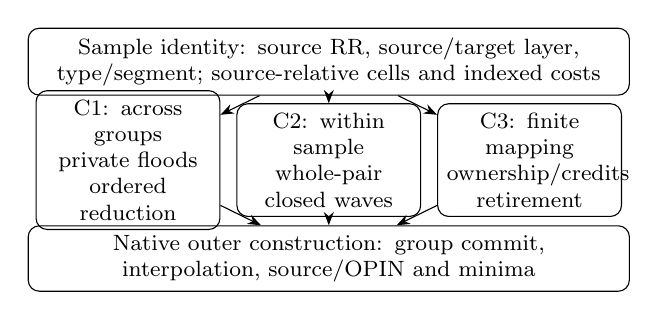
\begin{tikzpicture}[>=Stealth, every node/.style={draw,rounded corners,align=center,font=\footnotesize}]
\node[text width=7.4cm] (a) at (0,0) {Sample identity: source RR, source/target layer, type/segment; source-relative cells and indexed costs};
\node[text width=2.1cm] (s) at (-2.55,-1.25) {C1: across groups\\private floods\\ordered reduction};
\node[text width=2.1cm] (g) at (0,-1.25) {C2: within sample\\whole-pair\\closed waves};
\node[text width=2.1cm] (f) at (2.55,-1.25) {C3: finite mapping\\ownership/credits\\retirement};
\node[text width=7.4cm] (o) at (0,-2.5) {Native outer construction: group commit, interpolation, source/OPIN and minima};
\draw[->] (a)--(s);\draw[->] (a)--(g);\draw[->] (a)--(f);
\draw[->] (s)--(o);\draw[->] (g)--(o);\draw[->] (f)--(o);
\end{tikzpicture}
\caption{A common sample boundary with distinct semantic and implementation obligations. The FPGA outer interface is evaluated by replay and simulation, not board-integrated native timing.}\label{fig:contracts}
\end{figure}


\subsection{STRICT: Private Floods, Ordered Reduction}
Workers own reset-per-sample visited costs, expanded bits, queues and outputs; graph/cost data are shared read-only. Native X/Y/Z filtering, layer slices, bounding boxes and edge/cost operations remain unchanged.

The native smallest-entry rule replaces a populated cell only for a strictly smaller delay. Congestion belongs to the winning delay; it must not be minimized independently. The retained directed reduction check inserts $(1,3)$ then $(1,9)$ and detects a wrong last-tie choice: strict-delay insertion must retain $(1,3)$. Independent coordinate minima can also synthesize a pair never produced by a path. These are explanatory counterexamples, not weakened timing baselines. For finite occupied representatives, the winning sample is the earliest minimum-delay sample in native enumeration order:
\begin{equation}
j^*(u)=\arg\min_{j\,\mathrm{occupied}}(d_{g,j}(u),j).
\end{equation}
Implementation uses the native insertion and occupancy predicates, including missing-state behavior, rather than generic tuple sorting.

\begin{proposition}
If native sample selection and within-flood visitation are unchanged, valid recorded delays are finite, and final commits/interpolation follow native order, private sample execution followed by original-order strict-delay reduction yields the native wire-cost table.
\end{proposition}
\noindent\emph{Proof.} Each private flood produces the same per-cell representative as its native flood. Serial execution concatenates the visitation sequences in sample order. Original-order reduction selects the minimum delay and retains the earliest associated congestion on ties. Occupancy agrees cell by cell; identical commits and interpolation preserve that agreement. Task completion order does not enter the argument. $\square$

The proposition excludes changed heap ties, exceptional-value reassociation and altered recording contexts; it concerns wire maps, not routing trajectories.

Group executes samples concurrently but waits at each group boundary. Pipeline exposes all groups through a bounded stream with parallel search and original-order reduction; reusable private workspaces avoid repeated allocation. Flat is an independent globally flattened parallel-loop control, not VPR's separate flat-routing option. Interpolation within a slice retains native order.

\subsection{ALT: Whole-Pair FP32 Bucket Waves}
ALT\_BUCKET\_FP32\_V1 is a separate contract. Admitted costs and accumulated candidates must be positive normal FP32 values or positive zero (negative zero and subnormals are rejected); unsupported numerics or capacity failures return an error without publishing a partial map. Admission includes $N<2^{23}$. Labels initialize to infinity except source $(0,0)$; missing cells retain their missing state.

For labels $a,b$, strict improvement means
\begin{equation}
a\prec b\iff a_d<b_d\ \lor\ (a_d=b_d\land a_q<b_q).
\end{equation}
The entire pair is selected. For nonnegative finite floats, CUDA packs the delay bits above congestion bits in a 64-bit word, allowing an unsigned atomic minimum to select one actual pair. It never combines a delay from one path with congestion from another. FP32 additions use round-to-nearest with contraction disabled in the matched implementations.

Scheduling uses $B(d)=\mathrm{bits}_{32}(d)\gg s$. We fix $s=20$ for the native experiments. Shift coarsens scheduling buckets, not stored delays: labels and returned costs remain FP32. Shift zero uses exact FP32 delay keys, still with ALT tie semantics.

A wave selects the smallest pending bucket, filters stale notifications and takes the current labels as its snapshot. All eligible outgoing edges generate proposals from that snapshot. Per-destination proposals begin from the existing label and reduce whole pairs; labels are committed only after expansion completes. Strictly improved destinations are published to their new bucket, including reinsertion into the current bucket. Pending deduplication avoids losing same-bucket notifications; old notifications are filtered on extraction. Closure occurs only when no pending work remains in the selected bucket. Target cells are recorded after closure, using whole-pair selection, and completion is tested then.

\begin{algorithm}[t]\caption{ALT wave contract (one logical sample)}\label{alg:alt}
\begin{algorithmic}[1]
\State Reset labels, pending state and outputs; publish source
\While{pending work exists and target cells incomplete}
\State Select minimum pending bucket $b$; filter stale members
\State Read wave-start labels; generate eligible proposals
\State Reduce each destination by whole-pair $\prec$
\State Commit strict improvements; publish or deduplicate
\If{bucket $b$ has no remaining work}
\State Record closed target cells; test target completion
\EndIf
\EndWhile
\State Return complete output or explicit failure
\end{algorithmic}\end{algorithm}

CPU uses a sparse directory and per-wave proposals; CUDA uses dense directory scans, parallel expansion, atomic proposals and launch barriers. Reset, synchronization and output handoff are charged. Finite iteration/work/capacity guards return failure rather than a partial successful map. Exhaustion or target completion after closure terminates the search. Whole-pair selection preserves association but does not prove a global lexicographic FP32 shortest-path theorem: rounding can erase an earlier delay difference. Table~\ref{tab:guarantees} summarizes the guarantees.

\begin{table}[t]\centering\caption{Semantic obligations and limits.}\label{tab:guarantees}
\begin{tabular}{lp{5.7cm}}\toprule Contract & Guarantee / boundary\\\midrule
STRICT & Native wire-map equality under unchanged samples, visitation, finite occupied delays and original-order reduction/interpolation.\\
ALT & Whole-pair wave rule and source-relative recording; native equality and universal QoR are not promised.\\
Finite ALT & Executed-case RTL/model agreement under declared service; physical timing and board memory are separate.\\\bottomrule\end{tabular}\end{table}

\section{Finite Heterogeneous Mapping}
The spatial ALT mapping connects 64 lanes in 16 frontend groups, 64 canonical banks and 32 shared memory ports. Samples execute sequentially at the batch controller. Runtime inputs supply source identities and target counts, never expected answers. Admission checks at most $2^{22}$ nodes, 32,768 cells, 256 samples, 32-bit line addresses and disjoint aligned regions. Descriptor/cost validation is a host invariant.

State ownership determines the pipeline. Initialization, cost loading and source seeding precede a finite directory/minimum tree; token reservation precedes canonical POP. Transaction, descriptor, ready and target queues remain independently finite. Registered request/return contexts retain source, kind, generation and local identity. A connectivity-specialized network implements only legal endpoint connections, with finite credits and backpressure. Four lanes per group produce FP32 whole-pair proposals.

Each bank reserves in-flight ownership through proposal read, comparison and writeback. Occupied-set enumeration feeds finite scratch storage: unspilled resident fragments bypass a scratch read; spilled fragments require a merge. Canonical storage supports eight live transactions per bank, excludes concurrent same-word updates and commits complete words. Publication enqueue and retirement differ: directory effects remain live through the actual response and deferred acknowledgment. Expansion fences wait for frontend, candidate, bank and network drain; final completion waits for output-write acknowledgments. Arithmetic width alone therefore cannot predict throughput.

The selected RTL replaces return selection with a 116-bit bank-selected word multiplexer; other DUT sources and sequential logic are unchanged. No capacity or modeled service advantage is added.

Complete production-size RTL executes all 8/12 samples of two native graphs in 157,312/268,916 baseline cycles with exact ALT outputs and complete retirement. Response jitter (0--16 cycles) and 14-of-19-cycle admission increase the second run to 276,758 cycles without changing outputs or transaction counts. Eleven invalid configurations issue no request.

Across baseline, stress and conservative service, 52 complete executions match the finite model in total cycles, 19 exclusive phases, ordered intervals, waves and request/return identities. Calibration includes the real registered frontend-idle visibility stage, not a fitted cycle offset. Full BNN40/LSTM40 models verify 160 complete outputs across two services, phase sums, finite capacities and transaction conservation. This is executed-case agreement, not universal formal or synthesized functional equivalence. Small-graph cycles are not extrapolated by graph size.

\section{Experimental Method and Evidence}
\subsection{Frozen Inputs, Cohorts and Resources}
We reuse completed solver experiments and add a bounded compatibility preflight; no new performance solver or EDA job is launched. The retained corpus separates legal full-flow runs from construction-only observations; capped route tails do not establish legality. GEMM and scaling cohorts are separate. Scheduling controls and native ALT use distinct, separately bound RRGs.

The BNN/small-input native cohort measures BNN and s38417 with Stock, Flat, ALT CPU and original ALT CUDA. A separate cohort measures LSTM seed2 with those arms plus Pipeline. LSTM was not used in preceding ALT tuning and was frozen before its own qualification/timing; it was not preselected before all ALT development.

LSTM is a same-family tuning holdout, previously used in the CPU study. It shares BNN's architecture but differs in netlist, placement and RRG. LSTM has 4,166,724 nodes and 40,142,314 edges; BNN has 4,102,608 nodes and 39,480,616 edges. Both use two layers, width120 and 40 samples, not independent architectures.

The baseline is VTR commit \texttt{0b912334fdd8}, release build with assertion level 2. Native ALT uses a Xeon Gold 6530 with eight distinct physical cores in one NUMA node and one H100 80GB, executing solvers sequentially. Shared instances are not exclusive. The LSTM cohort rotates arm order across three processes. Hosts/phases are not pooled.

\subsection{Timing and Statistical Policy}
E1 is sample service; the CUDA wrapper ends E1 before final ABI output copy. E2 is native \texttt{MapLookahead::compute}: conversion, preparation/service, output handoff, group merge, interpolation, source/OPIN and derived minima. Process adds RR XML loading, initialization, routing, checking/STA and uniform serialization. Independent route readback is outside Process; pre-generated RRG, packing and placement are excluded. Caches are not flushed.

For paired repeat $r$, $s_r=T_{c,r}/T_{a,r}$. We report mean and sample SD of these ratios and of raw seconds ($n=3$). SD is variability, not a confidence interval; repeats are processes, not designs or seeds. Stock E2 has 0.01-second precision; other E2 timers are high resolution. Profiles are outside formal timing.

\subsection{Qualification and Attribution}
STRICT checks native wire-map bytes under its proposition. ALT separately checks complete CPU/CUDA sample pairs and maps, then each candidate route through independent original-VPR FULL/STA readback with unchanged route SHA, zero overuse, and CPD/wirelength within $+5\%$ of control. LSTM uses both Flat and Stock controls.

Retained bounding-box notification repairs can change routing trajectories despite identical wire maps; a unique complete cause is not established. Stock ratios therefore describe the implementation combination. Shared-repair Flat/Pipeline/ALT comparisons better isolate construction.

\section{Results and System Interpretation}
\subsection{STRICT Cross-Sample Parallelism}
On eight-core GEMM, STRICT Pipeline reduces construction from 149.56 to 20.95 seconds and achieves $1.638\pm0.005\times$ paired Process speedup over Stock; Group takes 37.88 seconds. Construction is about 45\% of Stock Process. Existing sixteen-core GEMM full-flow records do not form a matched native CUDA cohort. Matched Group/Flat/Pipeline controls isolate C1 from other Stock repairs.

\begin{figure}[t]\centering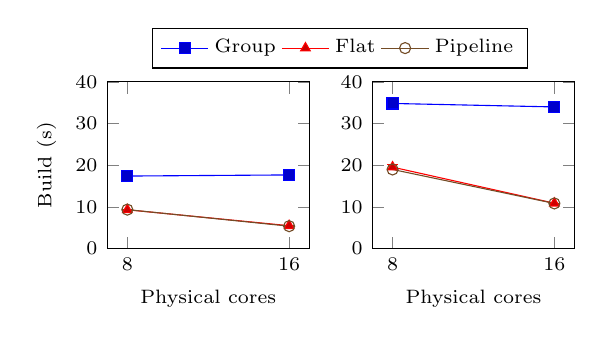
\begin{tikzpicture}
\begin{groupplot}[group style={group size=2 by 1,horizontal sep=0.8cm},width=4.15cm,height=3.7cm,xtick={8,16},xmin=7,xmax=17,ymin=0,ymax=40,xlabel={Physical cores},ylabel={Build (s)},label style={font=\scriptsize},tick label style={font=\scriptsize},legend style={font=\scriptsize,at={(1.15,1.08)},anchor=south,legend columns=3},error bars/y dir=both,error bars/y explicit]
\nextgroupplot[title={},ylabel={Build (s)}]
\addplot+[mark=square*] coordinates {(8,17.413333333333334) +- (0,0.3250128202599597) (16,17.683333333333334) +- (0,0.3257811126098835)};
\addplot+[mark=triangle*] coordinates {(8,9.32) +- (0,0.15394804318340596) (16,5.506666666666667) +- (0,0.030550504633038766)};
\addplot+[mark=o] coordinates {(8,9.363333333333333) +- (0,0.10598742063723142) (16,5.3933333333333335) +- (0,0.08082903768654771)};
\legend{Group,Flat,Pipeline}
\nextgroupplot[title={},ylabel={}]
\addplot+[mark=square*] coordinates {(8,34.82333333333333) +- (0,0.3181718613160717) (16,33.99) +- (0,0.6602272336097627)};
\addplot+[mark=triangle*] coordinates {(8,19.553333333333335) +- (0,0.6217180497084931) (16,10.896666666666667) +- (0,0.040414518843273746)};
\addplot+[mark=o] coordinates {(8,18.993333333333332) +- (0,0.11503622617824955) (16,10.846666666666668) +- (0,0.04041451884327389)};
\end{groupplot}
\end{tikzpicture}

\caption{Construction means and sample SD, three processes per arm/point. Same-cohort Group/Flat/Pipeline controls on BNN (left) and DLA (right); capped routing tails do not establish full-route legality. Error bars are small at this scale.}\label{fig:causal}\end{figure}

In Fig.~\ref{fig:causal}, ten groups of four samples limit group-local concurrency. At eight cores, BNN Group/Flat/Pipeline take $17.41\pm0.33$, $9.32\pm0.15$ and $9.36\pm0.11$ s. Flat and Pipeline independently remove barriers and are nearly equal: the benefit comes from decoupling groups, not a particular Pipeline primitive. At sixteen cores Flat/Pipeline take 5.51/5.39 s, against Group's 17.68 s. DLA shows the same mechanism (34.82/19.55/18.99 s at eight cores). Separate 2D controls also benefit: eight-core BNN-2D takes 7.75/4.23/4.16 s. These are not equal-sized 2D/3D pairs, so layer count is not a causal explanation of time differences.

\subsection{Wave Scheduling: Concurrency Versus Work}
\begin{table}[t]\centering\caption{Matched BNN40 original-representation profiles; diagnostic operation counts, not native E2 timing.}\label{tab:waves}
\begin{tabular}{lrr}\toprule Metric & Shift 0 & Shift 20\\\midrule
\tableinput{tables/waves.tex}\bottomrule\end{tabular}\end{table}
Table~\ref{tab:waves} recomputes complete per-sample profiles. Shift 20 reduces summed waves by $9.112\times$ and maximum per-sample waves (the corresponding batch rounds) by $10.627\times$, while increasing eligible edge work only $0.3504\%$. Edge-work-weighted frontier grows $6.6484\times$. This exposes more work per synchronization opportunity; it is neither an occupancy measurement nor proof that launches explain all runtime. Labels remain FP32 and shift-0/20 complete CPU/CUDA outputs agree under ALT. Instrumented profile times are excluded from native statistics. Retained fixture checks include eight random cases with native congestion differences, motivating separate semantic/QoR qualification.

\subsection{Native LSTM: Optimized CPU and Matched ALT}
\begin{table}[t]\centering\caption{LSTM native seconds, mean $\pm$ sample SD ($n=3$); one rotated cohort, eight CPU cores and one H100.}\label{tab:lstm}
\begin{tabular}{lrr}\toprule Method & E2 & Process\\\midrule
\tableinput{tables/lstm.tex}
\bottomrule\end{tabular}\end{table}

CUDA obtains \LstmPipeBuild\ E2 and \LstmPipeProc\ Process acceleration against Pipeline; against Flat, \LstmFlatBuild\ and \LstmFlatProc; against matched ALT CPU, \LstmAltCpuBuild\ and \LstmAltCpuProc.  ALT CPU is close to Pipeline: changed search semantics alone do not explain GPU acceleration.

The smaller Process gain reflects remaining loading, initialization, routing and checking.

\subsection{Semantics, QoR and Size Dependence}
\begin{table}[t]\centering\caption{LSTM qualification objects. Map-word differences are against Flat.}\label{tab:qor}
\begin{tabular}{lr}\toprule Object / metric & Observation\\\midrule
\tableinput{tables/qor.tex}
\bottomrule\end{tabular}\end{table}

ALT CPU/CUDA agree on complete samples and maps, but have different route SHAs; each independently passes readback. ALT changes 23,111 congestion words against Flat with no delay or missing-state changes (Table~\ref{tab:qor}). Native strict-delay ties and ALT whole-pair improvement remain different contracts.

\begin{table}[t]\centering\caption{BNN/small-input Flat/ALT CUDA paired speedup, mean $\pm$ sample SD ($n=3$). Separate worker from LSTM.}\label{tab:legacy}
\begin{tabular}{lrr}\toprule Case & E2 speedup & Process speedup\\\midrule
\tableinput{tables/legacy.tex}
\bottomrule\end{tabular}\end{table}

BNN supplies another large native result against Flat; Pipeline supplements from another worker cannot create a matched BNN Pipeline/CUDA comparison.

The s38417 slowdown is retained: device initialization, scans and launches can outweigh a small build. ALT CPU helps construction, while Stock is fastest for full Process in this cohort. No automatic size selector or all-size benefit is established.

\subsection{Closest Alternative and Cache Applicability}\label{sec:applicability}
The locked executable exposes \texttt{compressed\_map} and map read/write options. Its embedded assertion and compute source explicitly require one layer; audited BNN/LSTM graphs have two. This is a static domain exclusion, not a measured failed 3D run or infinite runtime. The compressed reader and binary writer are also unimplemented (CSV export is separate). We do not upgrade VTR and infer no performance superiority over supported compressed-map configurations. Separable is also exposed by locked-binary help, but was not qualified or timed here.

For ordinary map caching, 36 retained formal reuse records have legal routing and independent FULL/STA checks on fixed inputs. They establish valid cache hits, separate from fresh construction. No unobserved cross-design reuse is amortized. No independent CPU quota was available for new formal timing; existing complete profiles avoid another shift sweep.

\section{Conditional Resident and Physical Evaluation}
\subsection{A Separate Optimized Software Cohort}
Resident completion includes state initialization, cost loads, all waves, canonical/directory retirement, output writes and acknowledgment drain. Host preparation and full readback are separate. This boundary differs from native E2 and Process. We reuse an affinity/NUMA-bound packed CPU implementation on dual Xeon Gold 6530 processors, testing 8, 32 and 64 workers. The 64-worker setting minimizes mean resident time on both full 40-sample workloads. The allocation has 64 physical cores and a 55-CPU-time quota; 40 samples permit at most 40 concurrent solves. This is the strongest measured CPU here.

Three independent processes each execute one warmup and three formal repetitions. Table~\ref{tab:resident} reports the mean and sample SD of the three process means, not nine independent trials. H100 resident includes initialization, launches/control, completion reads and synchronization; full output transfer and research comparison are outside. The BNN GPU receipt lacks an execution-time executable digest; its source/build provenance is a documented limitation.

\begin{table}[t]\centering
\caption{Complete-batch resident software time (seconds). CPU dispersion is over three independent process means. This cohort is separate from native eight-core E2/Process.}\label{tab:resident}
\setlength{\tabcolsep}{4pt}
\begin{tabular}{lrr}\toprule & BNN40 & LSTM40\\\midrule
CPU (64 workers) & $0.699624\pm0.026647$ & $0.725510\pm0.021287$\\
Retained H100 mean & 0.151800 & 0.159498\\
\bottomrule\end{tabular}
\end{table}

\subsection{Finite Model: Assumed Frequency and Memory}
We evaluate a \emph{hypothetical 200 MHz core} with declared 32-byte memory service. Baseline latency/issue interval is 80/5 ns; a conservative sensitivity scenario uses 160/10 ns. These correspond to 16/1 and 32/2 cycles at the assumed frequency. Reads and writes share the 32 physical ports; finite queues, credits, return identity and blocking remain active. Issue ceilings of 204.8/102.4 GB/s are not measured HBM throughput; conservative is not worst-case.

\begin{table}[t]\centering
\caption{Complete finite-model results at \emph{assumed 200 MHz}; neither routed-frequency performance nor board measurement.}\label{tab:model}
\begin{tabular}{llrr}\toprule Case & Latency/issue & Cycles & Model s\\\midrule
BNN40 & 80/5 ns & 102,557,024 & 0.512785\\
LSTM40 & 80/5 ns & 104,154,414 & 0.520772\\
BNN40 & 160/10 ns & 135,128,351 & 0.675642\\
LSTM40 & 160/10 ns & 137,198,248 & 0.685991\\
\bottomrule\end{tabular}
\end{table}

These deterministic predictions have no sampling error bars. Baseline expansion consumes 77.09/77.15\% of BNN/LSTM cycles and finalization 20.95/20.89\%; all other mutually exclusive phases account for the remainder. Candidate throughput is about 25.4\% of the 64-lane ideal: finite scheduling, transport and publication constrain parallelism. Overlapping stall counters are not additive.

The conservative BNN prediction exceeds the fastest measured CPU process mean, 0.668921 s, despite lying below its three-process mean. Thus the conditional result does not establish robust CPU superiority; GPU is faster in both scenarios. Frequency changes alter service discretization and scheduling: $T=C(f,\text{service},\text{structure})/f$, with absolute nanoseconds rounded up to cycles. Dividing old cycles by a new frequency is invalid when that binding changes.

Resident predictions exclude host preparation/readback and native assembly. Packed descriptors are shared by selected CPU/FPGA representations. Host layout conversion is not board DMA; unrelated native cohorts cannot supply an end-to-end FPGA speedup.

\subsection{Actual Full-Core Physical Status}
\begin{table}[t]\centering
\caption{Actual full-core resources on XCU280, Vivado 2022.2. Failed routing rows are error-checkpoint resources, not completed routes. BRAM is in 36-Kb equivalents; all rows use 640 URAM and zero DSP.}\label{tab:physical}
\begin{tabular}{lrrr}\toprule Stage & LUT & FF & BRAM\\\midrule
Final RTL synthesis & 1,223,270 & 749,607 & 1,148\\
Final RTL standard opt & 1,220,068 & 748,933 & 1,148\\
Final RTL placement & 1,212,828 & 749,091 & 1,148\\
Prior default route failure & 1,233,715 & 749,174 & 1,148\\
Prior SSI route failure & 1,232,534 & 749,226 & 1,148\\
\bottomrule\end{tabular}
\end{table}

The complete connected XCU280 core excludes the board shell, PCIe and memory controller. Standard optimization removes 3,202 LUTs and 674 FFs. Post-opt LUT use is 93.59\%: 932,268 logic LUTs, 286,776 LUTRAM and 1,024 SRLs. Placement uses 1,212,828 LUTs (925,700 logic, 286,232 LUTRAM, 896 SRL), but occupies 99.86\% of CLB sites. All 64 banks, 16 frontends, 32 ports and 9,681 nonconstant output bits remain, with no black boxes.

The predecessor fails default and SSI routing with approximately 5.8 million trial-routing overlaps. Its SSI failure checkpoint has setup WNS $-15.487$ ns and hold WHS $-3.530$ ns; the worst reported setup path crosses three SLR boundaries from bank completion payload to dispatcher error state. This motivates the single return-word selection change, not greater parallelism. Failure-checkpoint slack is not an achieved period.

In the read-only November 17 snapshot, placement, post-place reports and physical optimization have completed; routing is in progress. No qualified full-core frequency is established. The 5 ns constraint is a target. Post-opt sequential clock pins connect to the core clock; reset BUFG has zero clock loads. Placement buffers require connectivity classification; methodology/reset warnings and unproven constant aliases remain qualification obligations. FPGA execution time and CPU/FPGA speedup at an achieved frequency are consequently unavailable. The model above is neither board measurement nor a physical success claim.

\section{Scope and Limitations}
STRICT equality requires the stated order/numeric conditions; ALT qualification covers tested routes, not arbitrary graphs or a universal QoR bound. Same-family LSTM and repeated timings do not enlarge the architecture population. Shared instances and three processes limit small-difference claims. Hardware evidence establishes finite behavior and executed-case agreement, not board operation or measured memory service. Physical timing, shell integration and external-memory qualification remain separate; failed configurations do not establish universal FPGA limits.

\section{Conclusion}
Source context can survive group and search-order decoupling. STRICT separates private sample execution from native-order reduction; ALT separately specifies whole-pair FP32 waves and closure. Native LSTM CUDA achieves \LstmPipeBuild\ construction and \LstmPipeProc\ Process acceleration against eight-core Pipeline. Small-input slowdowns, representative differences and the same-family holdout scope delimit the result. RTL/model agreement extends the analysis under declared memory assumptions; full-core timing and FPGA superiority remain unestablished.

\section*{Content Generated by AI}
OpenAI Codex (GPT-6) assisted manuscript text/figures, artifact scripts, prior RTL/model development and experiments. Authors are responsible for verification and submission.

\clearpage
\bibliographystyle{IEEEtran}
\bibliography{references}
\end{document}
